\documentclass{beamer}

\usetheme{Frankfurt}
\beamertemplatenavigationsymbolsempty
\setbeamertemplate{footline}[frame number]

\usepackage[ngerman]{babel}
\usepackage[babel]{csquotes}
\usepackage[utf8]{inputenc}
\usepackage{listings}
\usepackage{color}
\definecolor{darkgray}{rgb}{0.4, 0.4, 0.4}
\definecolor{purple}{rgb}{0.65, 0.12, 0.82}
\definecolor{darkgreen}{cmyk}{0.7, 0, 1, 0.5}

\lstset{
  language=Python,
  basicstyle=\ttfamily,
  keywordstyle=\color{blue}\bfseries,
  ndkeywordstyle=\color{darkgray}\bfseries,
  identifierstyle=\color{black},
  commentstyle=\color{purple}\ttfamily,
  stringstyle=\color{red}\ttfamily,
  showspaces=false,
  showstringspaces=false,
  showtabs=false,
  framesep=2mm,
  tabsize=4,
  captionpos=b,
  breaklines=true,
  breakatwhitespace=true,
  numberbychapter=false,
  aboveskip=0.25cm,
  belowskip=0.25cm,
  inputencoding=utf8
}

\usepackage{graphicx}
\usepackage{hyperref}

\urlstyle{same}
\hypersetup{pdfpagemode=FullScreen,pdfpagelayout=SinglePage,pdfstartview=Fit}

\date{19.12.2012}
\subject{Webapplikationen mit Flask}
\title{Webapplikationen mit Flask}
\author{Adrian Mönnich}
\institute[Hochschule Karlsruhe]{
  Fakultät für Informatik und Wirtschaftsinformatik\\
  Hochschule Karlsruhe
}



\begin{document}
\maketitle
\section*{Überblick}
\frame{\tableofcontents}


\section{Motivation}
\begin{frame}
  \frametitle{Motivation}
  
\includegraphics[width=0.6\textwidth]{images/python-logo.png} \hspace*{\fill}
  \newline
  \hspace*{\fill} 
\includegraphics[width=0.5\textwidth]{images/flask-logo.pdf}
\end{frame}


\section{Python}
\begin{frame}[fragile]
  \frametitle{Python}
  \begin{itemize}
    \item Dynamische Programmiersprache
    \item Oftmals als Skriptsprache genutzt
    \item Mehrere Paradigmen
    \item Blöcke werden durch Einrückung definiert
  \end{itemize}

  \begin{exampleblock}{Python-Code}<2>
    \begin{lstlisting}
def hello_world():
    if False:
        print 'World demise on 2012-12-21.'
    print 'Hello World.'
    \end{lstlisting}
  \end{exampleblock}
\end{frame}

\begin{frame}[fragile]
  \frametitle{WSGI}
  \begin{itemize}
    \item Web Server Gateway Interface
    \item Python-Standard PEP-333: \url{http://www.python.org/dev/peps/pep-0333}
    \item Schnittstelle zwischen Webservern und Python-Applikationen
    \item WSGI-Applikationen sind \emph{callables} (also z.B. Funktionen)
  \end{itemize}
  \begin{exampleblock}{Hello WSGI}<2>
    \begin{lstlisting}
def application(environ, start_response):
    start_response('200 OK', [('content-type', 'text/plain')])
    return ['Hello World!']
    \end{lstlisting}
  \end{exampleblock}
\end{frame}

\section{Flask}
\begin{frame}
  \frametitle{Allgemeines}
  \begin{itemize}
    \item Microframework für Webapplikationen
    \item Sehr komfortabel zu nutzen - \enquote{Flask is Fun}
    \item Ausführliche Dokumentation
    \item \enquote{based on Werkzeug, Jinja 2 and good intentions}
    \item Open Source (BSD-Lizenz)
  \end{itemize}

  \begin{block}{BSD-Lizenz}<2>
    \begin{itemize}
      \item Kopieren, Verändern, Weitergeben ist erlaubt
      \item Copyright-Vermerk des Originals darf nicht entfernt werden
      \item Änderungen können unter einer beliebigen Lizenz veröffentlich werden (auch proprietär)
    \end{itemize}
  \end{block}
\end{frame}

\begin{frame}
  \frametitle{Aufbau}
  \begin{itemize}
    \item Application: Zentrale Klasse und WSGI-Anwendung (implementiert \lstinline{__call__()})
    \item Blueprints: Module, die eigene Routen, Templates, etc. enthalten können. Erlaubt bessere
          Strukturierung einer komplexeren Anwendung
    \item Routing: Mapping von URLs auf Python-Funktionen
    \item Sessions: Signierte Cookies
    \item Templates (Jinja 2)
    \item Signals: Hooks um z.B. vor jedem Request Code auszuführen
  \end{itemize}
\end{frame}

\begin{frame}
  \frametitle{Werkzeug}
  \begin{itemize}
    \item \enquote{WSGI utility library}
    \item Debugger
    \item Request/Response-Klassen
    \item Hilfsfunktionen für HTTP (Cookies, Dateiuploads, \ldots)
    \item URL-Routing
    \item \url{http://werkzeug.pocoo.org}
  \end{itemize}
\end{frame}

\begin{frame}
  \frametitle{Jinja 2}
  \begin{itemize}
    \item Templateengine
    \item Unterstützt Unicode/UTF-8
    \item Kompiliert Templates zu Python-Bytecode
    \item Vererbung
    \item Optionale Sandbox
    \item Autoescaping (HTML)
    \item \url{http://jinja.pocoo.org}
  \end{itemize}
\end{frame}

\section{Flask-Tutorial}

\begin{frame}
  \frametitle{Zielsetzung}
  \begin{itemize}
    \item Ein einfaches Feedback-Formular zu Flask selbst
    \item Zufrieden/unzufrieden inkl. kurzer Begründung
    \item Real existierende Applikation: \url{http://feedback.flask.pocoo.org}
    \item Quellcode: \url{https://github.com/mitsuhiko/flask-feedback}
  \end{itemize}

  \begin{exampleblock}{Screenshot}
    \begin{center}
      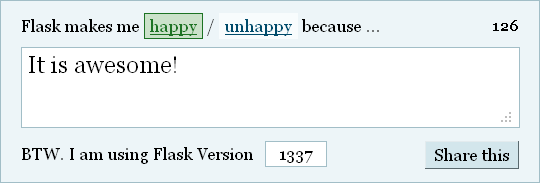
\includegraphics[width=0.5\textwidth]{images/flask-feedback.png}
    \end{center}
  \end{exampleblock}
\end{frame}

\begin{frame}
  \frametitle{Wieso ein Feedbackformular?}
  \begin{itemize}
    \item Einfache Applikation; hier jedoch weiter vereinfacht
    \item Datenbankanbindung
    \item Benutzerdaten (prinzipiell nicht vertrauenswürdig!)
    \item Nur wenige Python-Packages bzw. Flask-Extensions benötigt
  \end{itemize}
\end{frame}

\begin{frame}
  \frametitle{Flask-Extensions}
  \begin{itemize}
    \item Erinnerung: Flask ist ein Microframework
    \item Zusätzliche Funktionalität durch Erweiterungen
    \item Flask-SQLAlchemy: Einbindung des Datenbankframeworks \emph{SQLAlchemy}
    \item Flask-Script: Kommandozeilenbefehle
    \begin{itemize}
      \item Dev-Server inkl. Debugger
      \item Python-Shell
      \item Benutzerdefinierte Befehle (oftmals \emph{createdb} und \emph{dropdb})
    \end{itemize}
  \end{itemize}
\end{frame}

\end{document}
